\documentclass[11pt]{scrartcl}
\usepackage[a4paper]{geometry}

\usepackage{graphicx}
%\graphicspath{ {./images/} }

\usepackage{fancyhdr}
\pagestyle{fancy}
\fancyhf{}
\fancyhead[L]{SPIROMETRIE} %Kopfzeile links
\fancyfoot[C]{\thepage}

\usepackage[utf8]{inputenc}
\usepackage{csquotes}
\usepackage[german]{babel}

\usepackage{setspace}

\usepackage{caption}
\usepackage{float}

\usepackage{hyperref}
\usepackage{pdfpages}

\hypersetup{
    pdftitle = {Spirometrie},
    pdfsubject = {Biomedizinischesystemtechnik Praktikum},
    pdfauthor = {Leona K{\"o}ck, Chris R{\"u}ttimann},
    pdfkeywords = {} ,
    pdfcreator = {pdflatex},
    pdfproducer = {LaTeX with hyperref}
}

\usepackage[
    style=apa,
    backend=biber,
    sortcites=false,
    sorting=none,
    hyperref=true,
    backref=false
]{biblatex}
\usepackage{amsmath}
\usepackage[T1]{fontenc}
%\addbibresource{test.bib}

\begin{document}
    \pagenumbering{Alph}
% ---------------------
% Titlepage
% ---------------------
    \begin{titlepage}
        \begin{center}
        {\LARGE OST Ostschweizer Fachhochschule}
            \\[1.5cm]
            \linespread{1.2}\large { Biomedizinischesystemtechnik Praktikum }

            \huge{\bfseries Spirometrie}
            \\%[1.5cm]
            \large{durchgef{\"u}hrt am 22. März 2021}
            \\[1.5cm]
   %         \linespread{1}
           
\includegraphics[width=8cm]{../images/ost_logo.eps}
           \\[1cm]
            {\small{Autoren}}\\
            {\Large{Leona K{\"o}ck}}\\
            {\Large{Chris R{\"u}ttimann}}
            \\[1cm]

            \vspace*{\fill}
            \large{\today}
        \end{center}

    \end{titlepage}

% ---------------------
% Abstract
% ---------------------
    \pagenumbering{Roman}
 %   \pdfbookmark[section]{Abstract}{abstract}
 %   \section*{Abstract}
    \addtocounter{section}{0}

 %   \pagebreak
    \setstretch{1.25}
% ---------------------
% Table of contents
% ---------------------
    \tableofcontents
    \pagebreak


% ---------------------
% Body
% ---------------------
    \pagenumbering{arabic}

    \section{Problem- und Zielvorstellung}
   
    \section{Problemlösung}

    \subsection{Vorbereitung}
   

    Für der Versuch wurden folgende Materialien benötigt:

    \begin{itemize}
        \item  PC mit Software (Patientandatenbank und Audiometrieprogramm)
        
    \end{itemize}
    Fragen beantworten:


    \subsection{Messung}
    
    \section{Ergebnisse}


    \subsection{Proband Chris Rüttimann}
  
    \pagebreak

    \subsection{Proband Leona Köck}

   
    \section{Kritik und Anregungen}
	% Was ned ob ma des brucht
    \pagebreak

    \section*{Eigenständigkeitserklärung}
    \addcontentsline{toc}{section}{Eigenständigkeitserklärung}

    Hiermit bestätigen wir, dass wir diesen Bericht selbstständig und ohne fremde Hilfe verfasst haben.
    Alle verwendeten Quellen wurden entsprechend dem APA-Standard gekennzeichnet.
    \\[3cm]


    \begin{figure}[H]
        
\includegraphics[width=4cm]{.././images/Unterschrift_Leona.png}
    \end{figure}
    \begin{tabular}{@{} l@{}}
        \hline \\
        \makebox[6cm]{Leona Köck}\\[2cm]
    \end{tabular}


    \begin{figure}[H]
        
\includegraphics[width=4cm]{.././images/Unterschrift_Chris.png}
    \end{figure}
    \begin{tabular}{@{} l@{}}
        \hline\\
        \makebox[6cm]{Chris Rüttimann}
    \end{tabular}

    \pagebreak
% ---------------------
% References
% ---------------------
    \printbibliography
    \addcontentsline{toc}{section}{Literaturverzeichnis}

% ---------------------
% List of figures
% ---------------------
%    \listoffigures
%    \addcontentsline{toc}{section}{Abbildungsverzeichnis}
%    \pagebreak

% ---------------------
% List of tables
% ---------------------
%\listoftables



% ---------------------
% Anhang
% ---------------------

\appendix

    \section{Messung 1 Chris}
    \label{sec:chris1}

    \begin{figure}[H]
        \hspace*{-3cm}
        \centering
        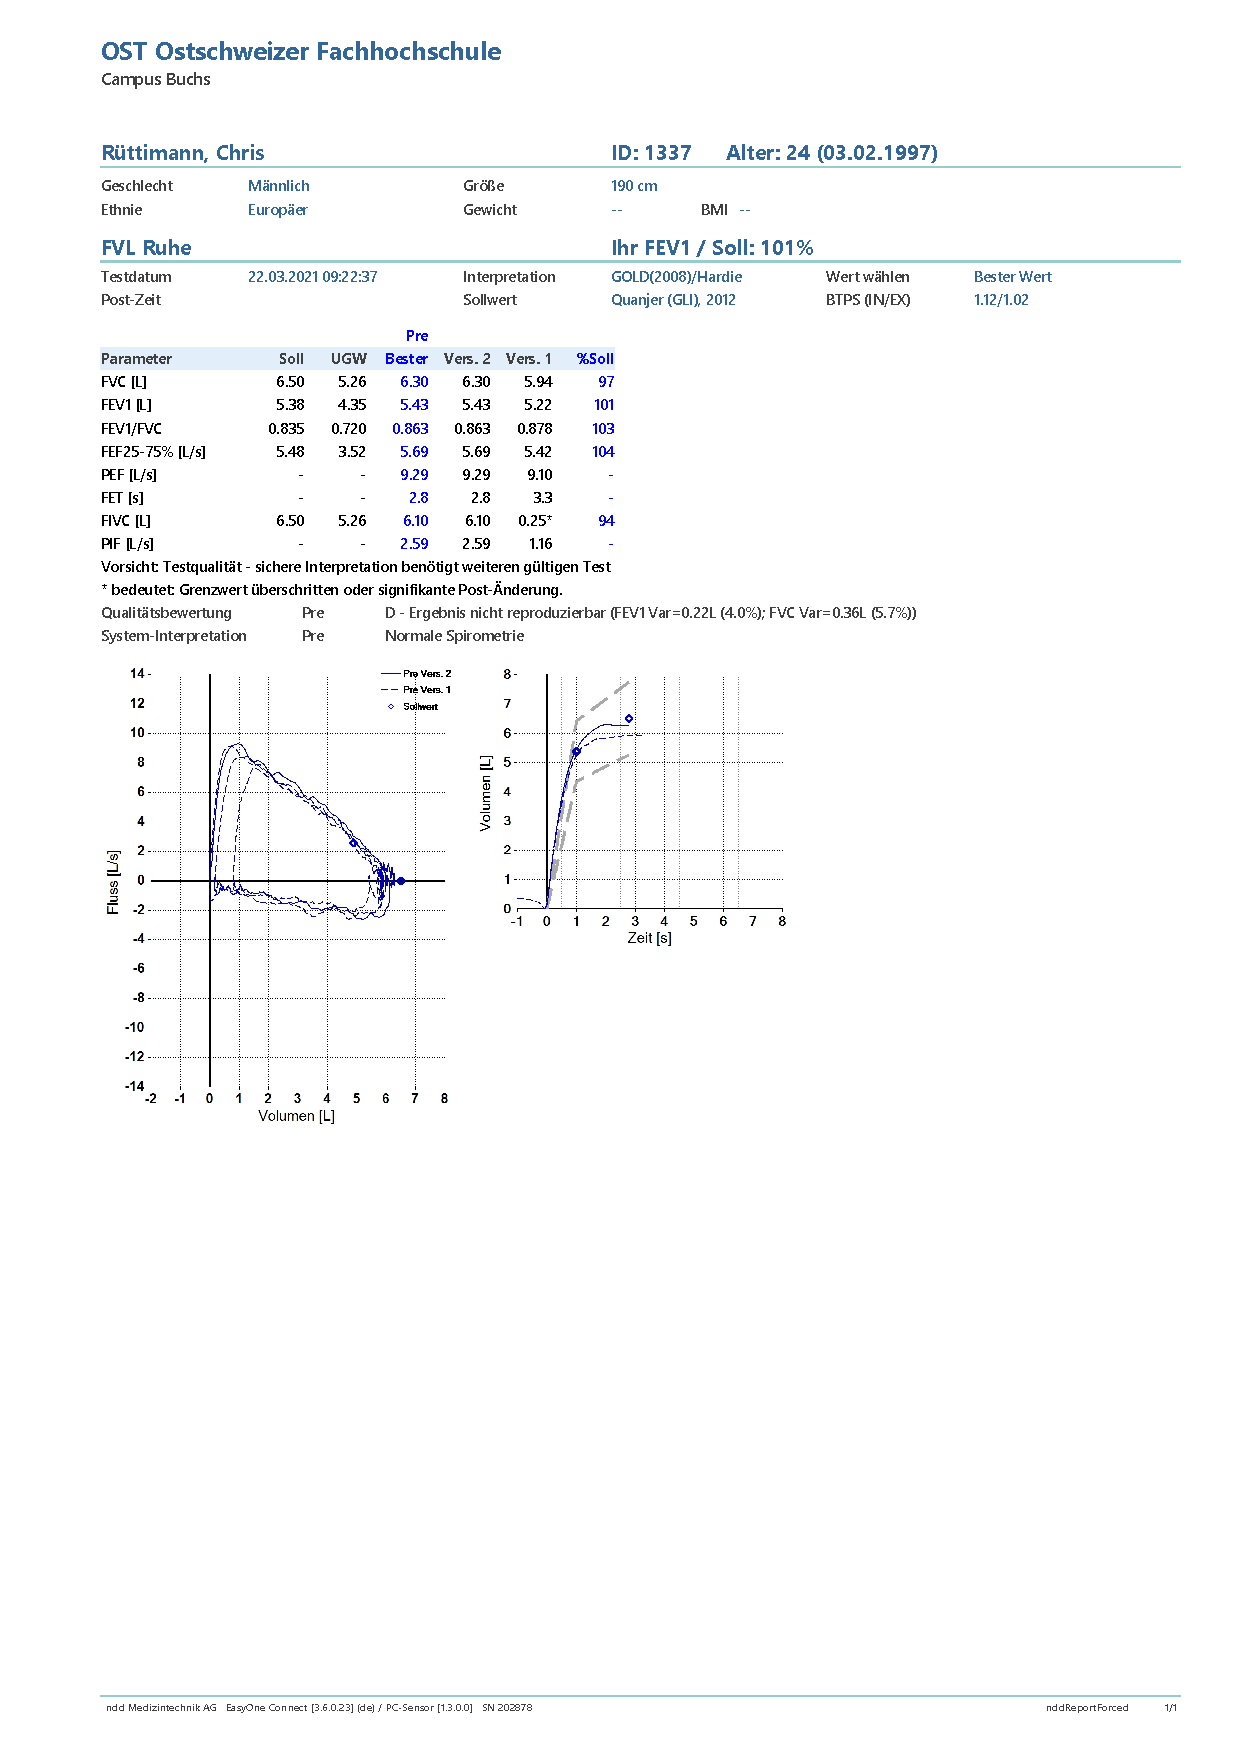
\includegraphics[clip, trim=0cm 13cm 0cm 0cm, width=1.4\textwidth]{Dateien/Chris1.pdf}
    \end{figure}

    \section{Messung 2 Chris}
    \label{sec:chris2}

    \begin{figure}[H]
        \hspace*{-3cm}
        \centering
        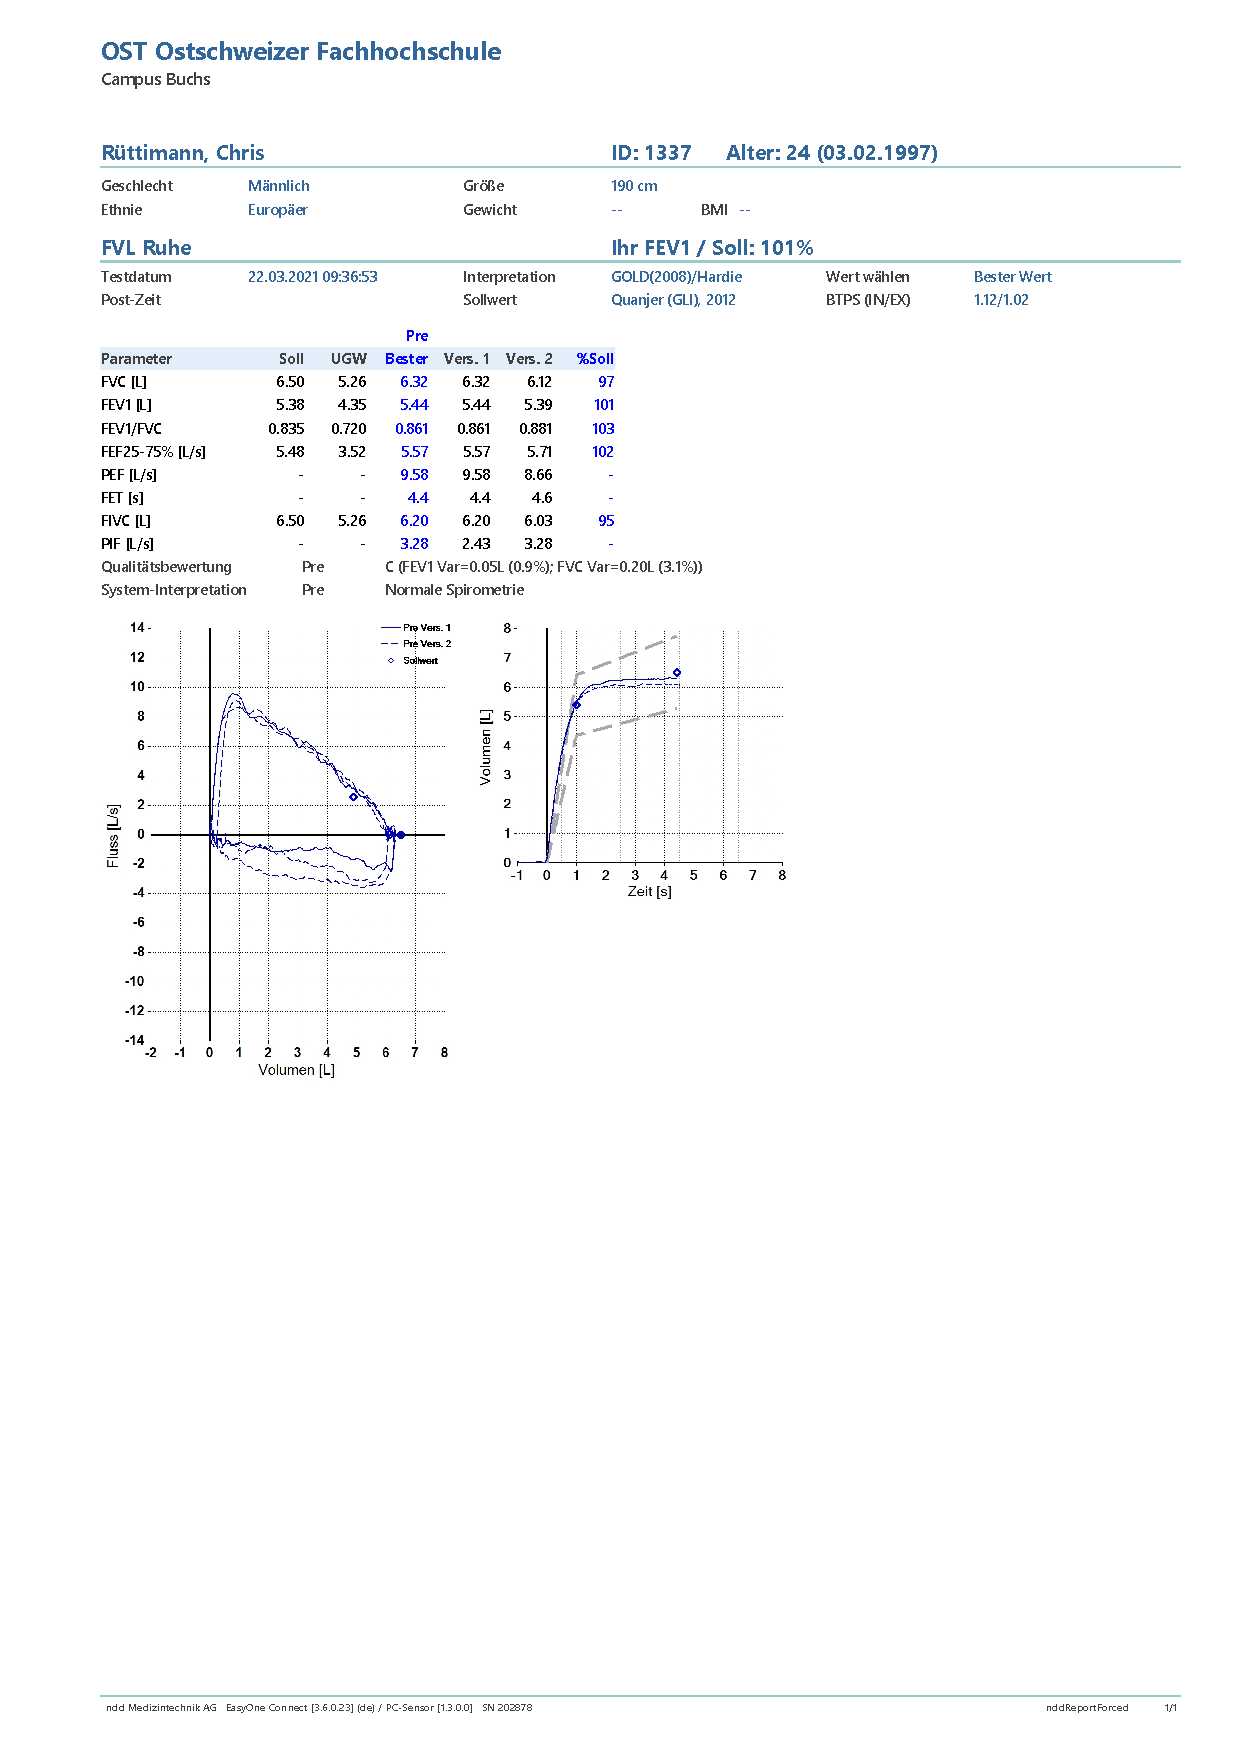
\includegraphics[clip, trim=0cm 13cm 0cm 0cm, width=1.4\textwidth]{Dateien/Chris2.pdf}
    \end{figure}

    \section{Messung 1 Leona}
    \label{sec:leona1}

    \begin{figure}[H]
        \hspace*{-3cm}
        \centering
        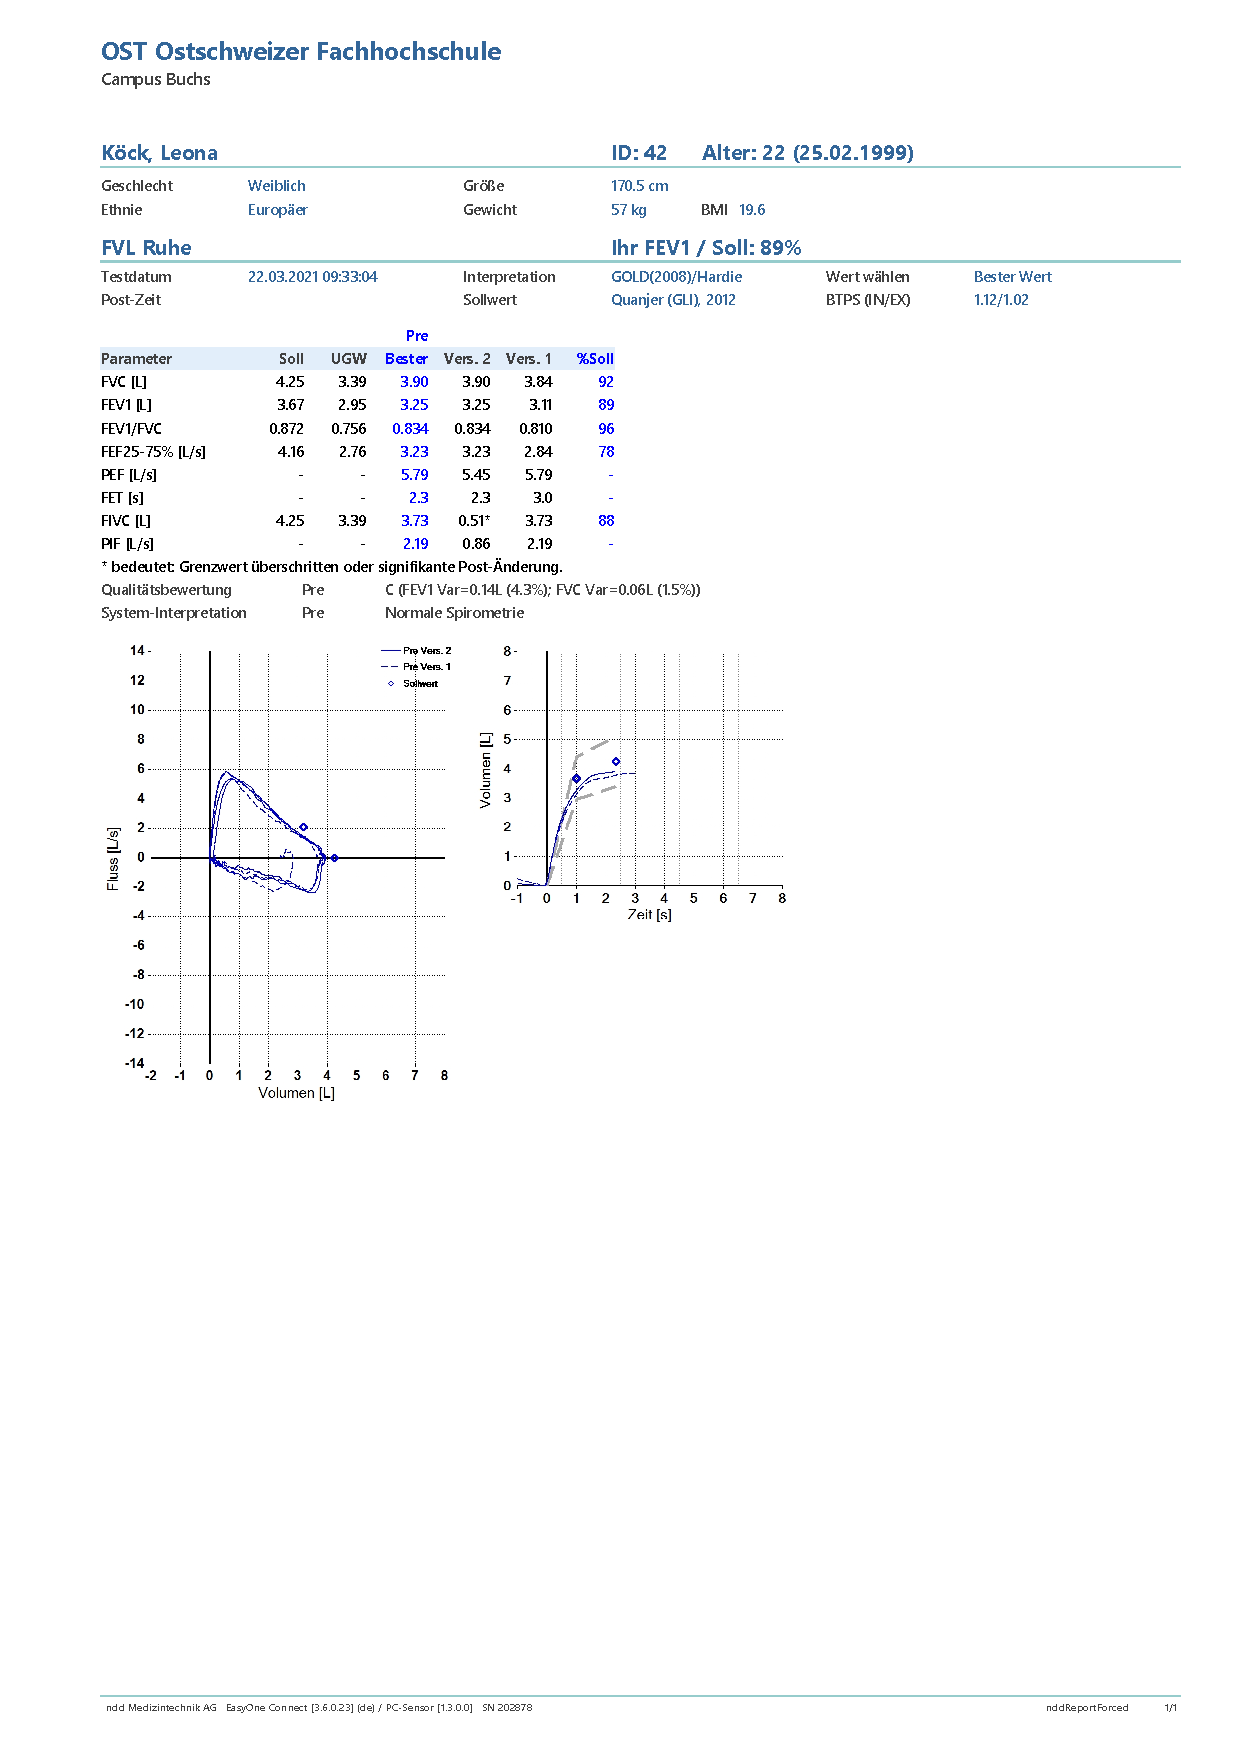
\includegraphics[clip, trim=0cm 13cm 0cm 0cm, width=1.4\textwidth]{Dateien/Leona1.pdf}
    \end{figure}

    \section{Messung 2 Leona}
    \label{sec:leona2}

    \begin{figure}[H]
        \hspace*{-3cm}
        \centering
        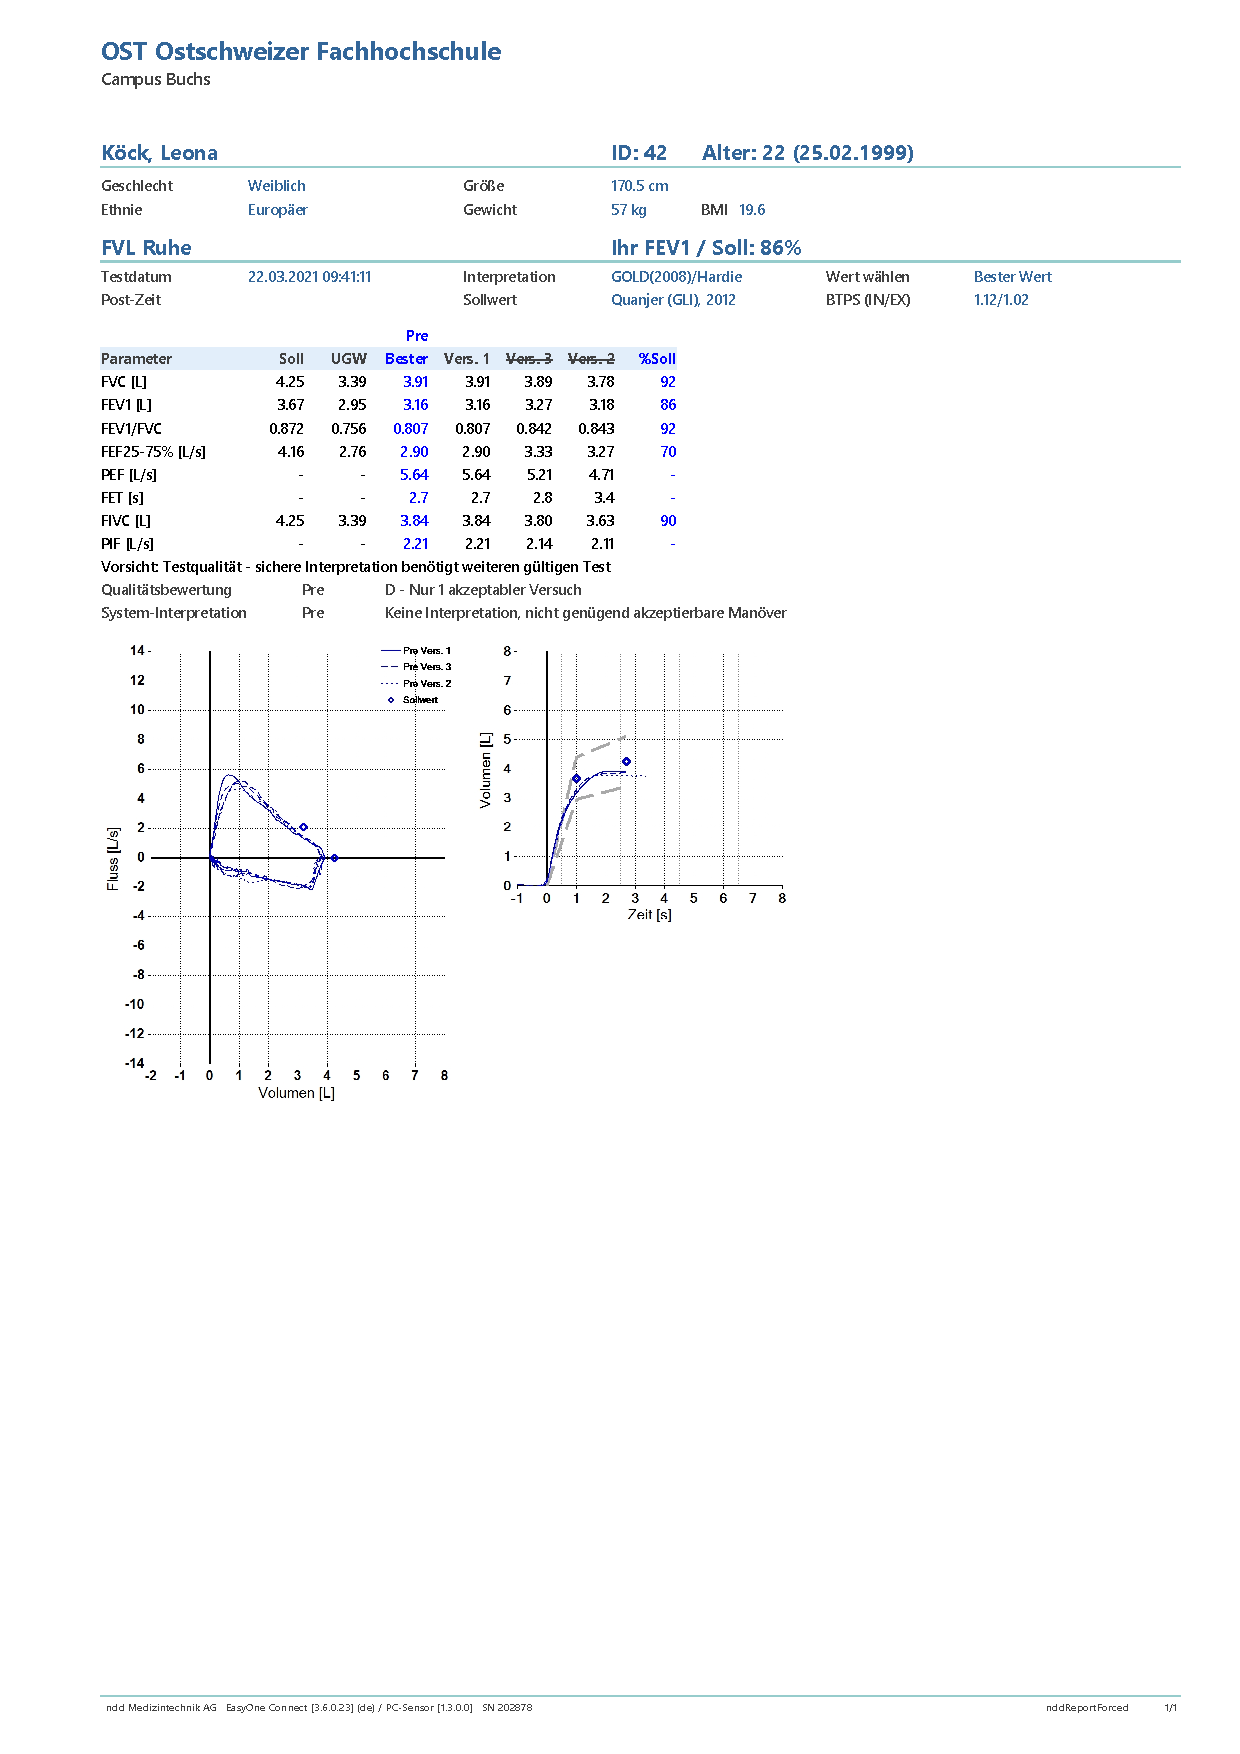
\includegraphics[clip, trim=0cm 13cm 0cm 0cm, width=1.4\textwidth]{Dateien/Leona2.pdf}
    \end{figure}

\end{document}